\documentclass[fleqn]{jbook}
\usepackage{physpub}

\begin{document}

\begin{question}{専攻 問題2}{}

\parbox[t]{110mm}{
三次元空間のある限られた領域(広がり幅を$a$とする)に電荷が分布し、
振動数$\nu$で振動している場合の電磁波の放射を考える。
右図のように座標をとって、電荷密度を$\rho(\vec{r},t)$、電流密度を
$\vec{j}(\vec{r},t)$とおくと、時刻$t$、観測点$\vec{R}$における
スカラーポテンシャル$\phi$とベクトルポテンシャル$\vec{A}$の遅延解は、
}\parbox[t]{55mm}{\vspace*{-10mm}
\begin{center}
  \mbox{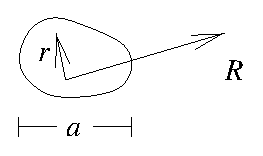
\includegraphics[clip]{1994phy2-1.eps}}
\end{center}}

%
\begin{eqnarray}
  \phi(\vec{R},t) &=& %
    \frac{1}{4\pi\varepsilon_0}%
    \int\frac{\rho(\vec{r},t-|\vec{R}-\vec{r}|/c)}%
    {|\vec{R}-\vec{r}|}\d{^3r} \eqname{1} \\
  \vec{A}(\vec{R},t) &=& %
    \frac{\mu_0}{4\pi}%
    \int\frac{\vec{j}(\vec{r},t-|\vec{R}-\vec{r}|/c)}%
    {|\vec{R}-\vec{r}|}\d{^3r} \eqname{2}
\end{eqnarray}
%
と書ける。ただし、$c$は真空中の光の速さ、$\varepsilon_0$と$\mu_0$
はそれぞれ真空の誘電率と透磁率である。式(1),(2)の積分で、時刻に関する
引数が``$t-|\vec{R}-\vec{r}|/c$"となっているのは位置$\vec{R}$、時刻
$t$における電磁波の強さが、電磁波の伝搬に必要な時間、
$|\vec{R}-\vec{r}|/c$、だけ前の時刻の電荷及び電流の分布に依存すること
を示している。

いま、電荷の分布している領域から観測点までの距離が電荷の広がりより
十分大きく($R \gg a$)、また、放射される電磁波の波長が電荷の広がりより
十分大きい($c/\nu \gg a$)場合を考える。このとき、式\eqhref{1}の積分に
おける電荷密度分布は、
%
\begin{equation}
  \rho(\vec{r},t-|\vec{R}-\vec{r}|/c)%
  \simeq \rho(\vec{r},t')%
  +\Partial{\rho}{t'}\frac{\vec{r}\cdot\vec{R}}{cR}  \eqname{3}
\end{equation}
%
と近似できる。ただし、$R\equiv|\vec{R}|,t'\equiv t-R/c$である。
さらに、$R \gg c/\nu$が満たされると、$\phi$と$\vec{A}$はそれぞれ、
%
\begin{eqnarray}
  \phi(\vec{R},t)%
    &\simeq& \frac{\int\rho(\vec{r},t')\d{^3r}}{4\pi\varepsilon_0R}%
         +\Partial{}{t'}\int\frac{\vec{R}\cdot\vec{r}\rho(\vec{r},t')}%
             {4\pi\varepsilon_0 cR^2}\d{^3r}%
    =       \frac{\int\rho(\vec{r},t')d^3r}{4\pi\varepsilon_0R}%
            +\frac{\vec{R}\cdot\dot{\vec{d}}(t')}%
             {4\pi\varepsilon_0cR^2} \eqname{4}\\
  \vec{A}(\vec{R},t)%
    &\simeq& \int\frac{\mu_0\vec{j}(\vec{r},t')}{4\pi R}\d{^3r}%
    =        \frac{\mu_0\dot{\vec{d}}(t')}{4\pi R} \eqname{5}
\end{eqnarray}
%
と近似できる。ただし、$\dot{\vec{d}}$\,は双極子モーメント
$\vec{d}(\equiv\int\vec{r}\rho \d{^3r})$を$t'(\equiv t-R/c)$に
ついて微分したものである。このとき、電場の強さ$\vec{E}$、磁束密度
$\vec{B}$は、それぞれ、
%
\begin{eqnarray}
 \vec{E} &=&%
   \frac{\mu_0\vec{R}\times(\vec{R}\times\ddot{\vec{d}})}{4\pi R^3}
    \eqname{6} \\
 \vec{B} &=&%
   \frac{\mu_0\ddot{\vec{d}}\times \vec{R}}{4\pi cR^2} \eqname{7}
\end{eqnarray}
%
と近似できる。ただし、$\ddot{\vec{d}}$\,は$\dot{\vec{d}}$\,を
$t'$について微分したものである。以下の問に答えよ。

\begin{subquestions}
\SubQuestion
  式\eqhref{3}を導け。

\SubQuestion
  式\eqhref{7}を導け。

\SubQuestion
\parbox[t]{100mm}{
  右図のように、$\ddot{\vec{d}}$\,を$z$軸方向、$\vec{R}$を$xz$平面内
  にとる。同様の図を描き、位置$\vec{R}$における電場$\vec{E}$と
  磁束密度$\vec{B}$の方向を図示せよ。さらに、ポインティングベクトル
  $\vec{P}$の方向も同じ図に書き込み、その大きさを$\theta$の関数として
  求めよ。ただし、$\ddot{\vec{d}}$\,と$\vec{R}$のなす角を$\theta$と
  する。
}\parbox[t]{60mm}{\vspace*{-20mm}
  \begin{center}
    \mbox{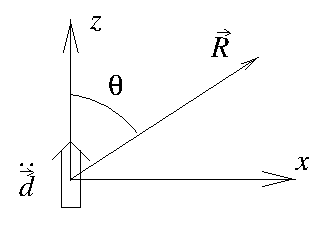
\includegraphics[clip]{1994phy2-2.eps}}
  \end{center}}

\SubQuestion
  単位時間あたりの全放射強度を求めよ。

\end{subquestions}
\end{question}
\begin{answer}{専攻 問題2}{}

\begin{subanswers}
\SubAnswer
  $R\gg a$、すなわち  $|\vec{R}|\gg|\vec{r}|$の条件では
%
  \[ \frac{|\vec{R}-\vec{r}|}{c} \simeq%
     \frac{R}{c} - \frac{\vec{R}\cdot\vec{r}}{cR} \]
%
  と近似できる。ところで、
  $\rho$の時間変化(すなわち$t$による変化)の周期は
  放射される電磁波の周期$1/\nu$ と同じ程度と考えられるが、
  $a/c \ll 1/\nu$ なので、$r/c$程度の時間での$\rho$の
  変化分は$\rho$の時間によるTaylor展開の$1$次の項で近似できる。
  よって、
%
  \[ \rho(r,t-|\vec{R}-\vec{r}|/c )%
     \simeq \rho(r,t-\frac{R}{c}+\frac{\vec{R}\cdot{\vec{r}}}{cR})%
     \simeq \rho(r,t')%
     +\Partial{\rho}{t'}\frac{\vec{R}\cdot{\vec{r}}}{cR} \]
%


\SubAnswer
  式\eqhref{5}で表されるベクトルポテンシャル $\vec{A}$に対して
  磁場 $\vec{B}$ は $\vec{B}=\Rot{\vec{A}}$である。
%
  \begin{eqnarray*}
    \partial_iA_j%
      &=& \frac{\mu_0}{4\pi R}\cdot%
          \ddot{d}\left(t-\frac{R}{c}\right)_j%
          \left(-\frac{1}{c}\right)%
          \left(\frac{R_i}{R}\right)%
        + \frac{\mu_0}{4\pi}\cdot%
          \dot{d}(t-\frac{R}{c})_j \frac{-R_i}{R^3} \\
      &=& - \frac{\mu_0}{4\pi cR^2}\cdot%
          R_i\cdot\left(\ddot{d}(t')_j+\frac{c}{R}\dot{d}(t')_j\right)\\
      \Yueni \Rot{\vec{A}} %
      &=& (\varepsilon_{lij}\partial_i A_j)%
       = - \frac{\mu_0}{4\pi cR^2}\cdot \vec{R}\times%
         \left(\ddot{\vec{d}}+\frac{c}{R}\dot{\vec{d}}\right)%
       = \frac{\mu_0}{4\pi cR^2}\cdot%
         \left(\ddot{\vec{d}}+\frac{c}{R}\dot{\vec{d}}\right)%
         \times\vec{R}
  \end{eqnarray*}
%
  となる。この$( )$の中の$2$つの項の大きさを比較する。
  $|\dot{\vec{d}}| \sim |\ddot{\vec{d}}|/\nu$ であるから
  後ろの項は
%
  \[ |\frac{c}{R}\dot{\vec{d}}(t')|%
     \sim \frac{c}{R\nu} |\ddot{\vec{d}}| \ll |\ddot{\vec{d}}| \]
%
  となるので前の項に対して無視できる。よって、
%
  \[ \vec{B} \simeq \frac{\mu_0}{4\pi}\frac{\ddot{\vec{d}}
                    \times\vec{R}}{cR^2} \]



\SubAnswer
\parbox[t]{95mm}{
  $\vec{B}\propto\vec{d}\times\vec{R}$で、$ \vec{d},\vec{R}$ともxz平面に
  平行なため、$\vec{B}$はxz平面に垂直。方向は紙面上から下。\\
  $\vec{E}\propto \vec{B}\times\vec{R}$となり、$\vec{B},\vec{R}$に
  垂直。
%
  \[ \vec{P}=\vec{E}\times\vec{H}%
     = \frac{\mu_0(\vec{R}\times(\vec{R}\times\ddot{\vec{d}}))\times
       (\ddot{\vec{d}}\times\vec{R})}{16\pi^2cR^5} \]
%
  方向は、$\vec{E}$と$\vec{H}$が互いに垂直のため、直ちに図の方向と
  わかる。大きさは、$\vec{R}$と$(\vec{R}\times\ddot{\vec{d}})$が
  垂直なので、
%
  \[ |\vec{R}\times(\vec{R}\times\ddot{\vec{d}})|%
     = |\vec{R}|^2|\ddot{\vec{d}}|\sin\theta \]
%
  となり、結局、
%
  \[ |P| = \frac{\mu_0R^3|\ddot{\vec{d}}|^2\sin^2\theta}{16\pi^2cR^5}
         = \frac{\mu_0|\ddot{\vec{d}}|^2}{16\pi^2cR^2}\sin^2\theta \]
%
  この様子を右図に記す。
%
}\parbox[t]{65mm}{
  \begin{center}
    \mbox{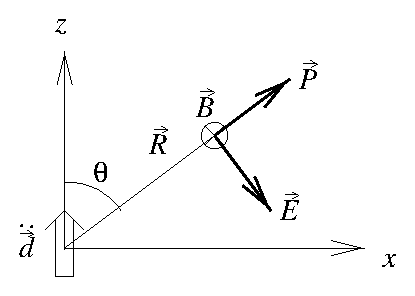
\includegraphics[clip]{1994phy2-3.eps}}
  \end{center}}


\SubAnswer
  {\bf 3}の$\vec{P}$は、原点を中心とする半径任意の球面に垂直である。
  よってfluxの総量は、$|\vec{P}|$をこの球面で積分すれば良い。
  全fluxをFとして、
%
  \[ F = R^2 2\pi \int_{0}^{\pi}|\vec{P}|\sin\theta \d{\theta}%
       = R^2 2\pi \frac{\mu_0|\ddot{\vec{d}}|^2}{16\pi^2cR^2}%
         \int_{-1}^{1}(1-\cos^2\theta)\d{\cos\theta}%
       = \frac{\mu_0|\ddot{\vec{d}}|^2}{6\pi c} \]

\end{subanswers}
\end{answer}



\end{document}
